\chapter{Introduction}


\section{Anatomy of Heart}
The function of the heart is to pump the blood inside the body, which is stimulated by an electrical stimulus. The heart pumps blood thorugh the arteries, veins to the different parts of the body such as organs, muscles and tissues.

The heart is made up of 4 chambers, left and right atria, and left and right ventricles,as can be seen in Figure ~\ref{fig:heart_anatomy}. The right atrium receives de-oxygenated blood from the whole body and pumps it into the right ventricle which then pumps the blood to the lungs for oxygenation. The left atrium receives oxygenated blood from the lungs and pumps it into the left ventricles which then pumps the oxygenated blood to the whole body. The aorta carries oxygenated blood to the different part of the body and the pulmonary arteries carry the de-oxygenated blood back to the lungs for oxygenation. The important point to note here is that, the blood flows to different organs via arteries and returns back to heart via veins.


The main components of the cardiac conduction system are:
\begin{enumerate}
	\item Synoatrial (SA) Node
	\item The Atrioventricular (AV) Node
	\item Atrioventricular (AV) Bundle or Bundle of His
	\item Right and Left Bundle Branches
	\item Purkinje Fibers
\end{enumerate}


\begin{figure}[htpb]
	\centering
	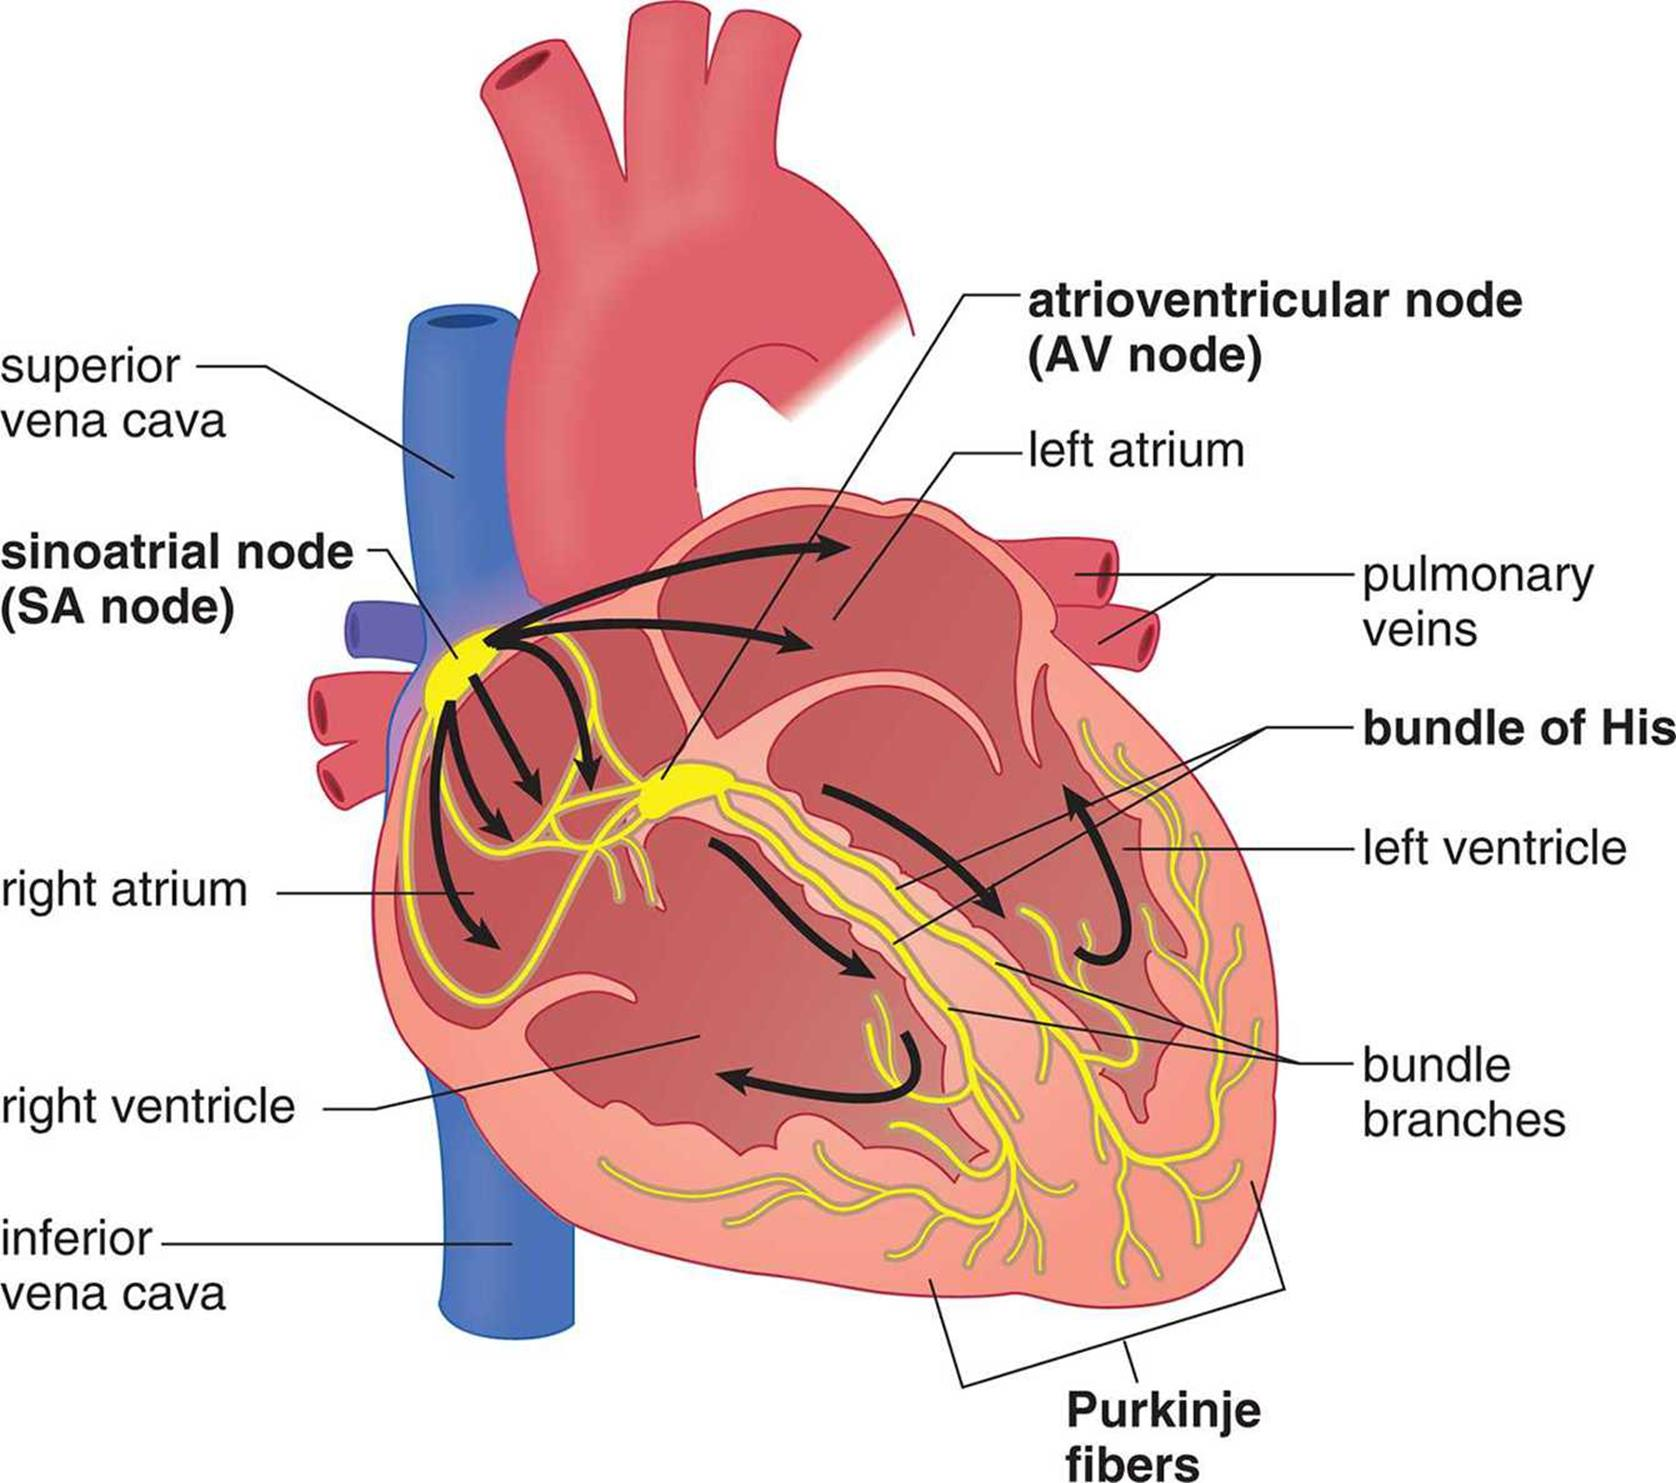
\includegraphics[width=\textwidth,height=7cm,keepaspectratio=true]{images/electric_activity_heart}
	\caption{
		The electrical activity of heart, taken from \cite{electric_activity_heart}.
	}
	\label{fig:heart_anatomy}
\end{figure}




The SA node, also known as sinus node, is a natural pacemaker of the heart which is located at the right atrium. It produces an electric stimulus at the rate of 60 to 100 signals per minute (under normal condition), which travels through the heart to make it pump the blood to the body. It initiates all heart beats and determine the heart rate. Electrical impulse from the SA node spread throughout the atrium which results in the contraction of the atrium. The AV node which is located on the other side of right atrium, near the AV valve. The purpose of this node is to serve as a gateway to the ventricles. It also delays the passage of electrical impulse to the ventricles. It is to ensure that, all the blood is ejected from the atria to the ventricles before the ventricles contract. The AV node then passes the signal to the atrioventricular (AV) bundle or bundle of His. The bundle is divided into two parts, right and left bundle branches to stimulate the right and left ventricles. The signal is then travels down to the Purkinje fibers where from the signal spreads upwards throughout the ventricular myocardium. Each contraction of the ventricles represents one single heartbeat.

Each heartbeat is composed of two phases, known as systole and diastole. During \textbf{systole}, the heat muscles contract and the blood is pumped from ventricles to the different parts of the body. During \textbf{diastole}, the hearts muscles relax and the blood from atria flows into the ventricles. The pressure generated during systole from the ventricular contraction is high, whereas, during diastole, the muscle relaxation reduces this pressure.

The electrical activity of the heart can be detected in the form of Electrocardiogram by placing electrodes on the body surface. It is a powerful tool for diagnosing the status of patient's heart.



\section{The Electrocardiogram} \label{the_electrocardiogram}

Electrocardiogram (ECG) is an essential tool for diagnosing the electrical activity of the heart. It is a simple, non-invasive procedure to measure the activity of the heart. Most of the tools available today to measure the ECG are based on the electrodes which are required to be attached to the body. The electrodes sense the electrical currents inside the body and transmit them to the ECG monitor. These currents are then transformed into appropriate waveforms which represent the heart's polarization and depolarization cycle. Different components of the wave represent activity of different parts of the heart.


In conventional 12-lead ECG, 10 electrodes or leads  are attached to the patient's body and then the electrical activity of heart is viewed from 12 different perspectives. These 12 views of heart are captured by placing the electrodes on chest, wrists, and ankles. The main purpose of ECG is to identify any cardiac arrhythmia, ischemia, problems with heart rate or irregularities.

These 10 electrodes are divided into 2 groups. 
\begin{enumerate}
	\item 6 chest electrodes
	\item 4 limb electrodes
\end{enumerate}

\begin{figure}[htpb]
	\centering
	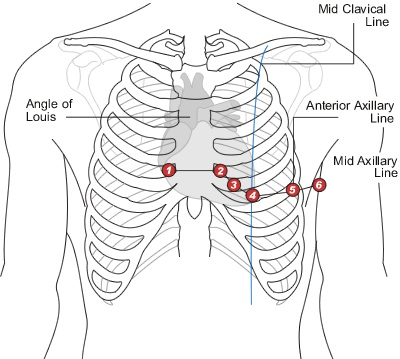
\includegraphics[width=\textwidth,height=6cm,keepaspectratio=true]{images/6_lead_placement}
	\caption{
		The leads position on chest, taken from \cite{TUON:six_leads}.
	}
	\label{fig:6_lead_placement}
\end{figure}


\subsubsection{Chest Electrodes}
The chest electrodes are denoted as ``V'' and they all are numbered from V1 to V6 as can be seen in Figure ~\ref{fig:6_lead_placement}. The electrodes are positioned at the following locations on the chest:

\begin{itemize}
	\item V1 - Fourth intercostal space (between ribs 4 and 5) on the right sternum
	\item V2 - Fourth intercostal space (between ribs 4 and 5) on the left sternum
	\item V3 - Placed in the middle of V2 and V4
	\item V4 - Fifth intercostal space (between ribs 5 and 6) at the mid-clavicular line
	\item V5 - Placed horizontally on anterior axillary line with V4
	\item V6 - Placed horizontally on Mid-axillary line with V4 and V5
\end{itemize} 


The 3 different axillary lines \textbf{anterior axillary line}, \textbf{midaxillary line}, and \textbf{posterior axillary line} can be seen in Figure ~\ref{fig:axillary_lines}. 

\begin{figure}[htpb]
	\centering
	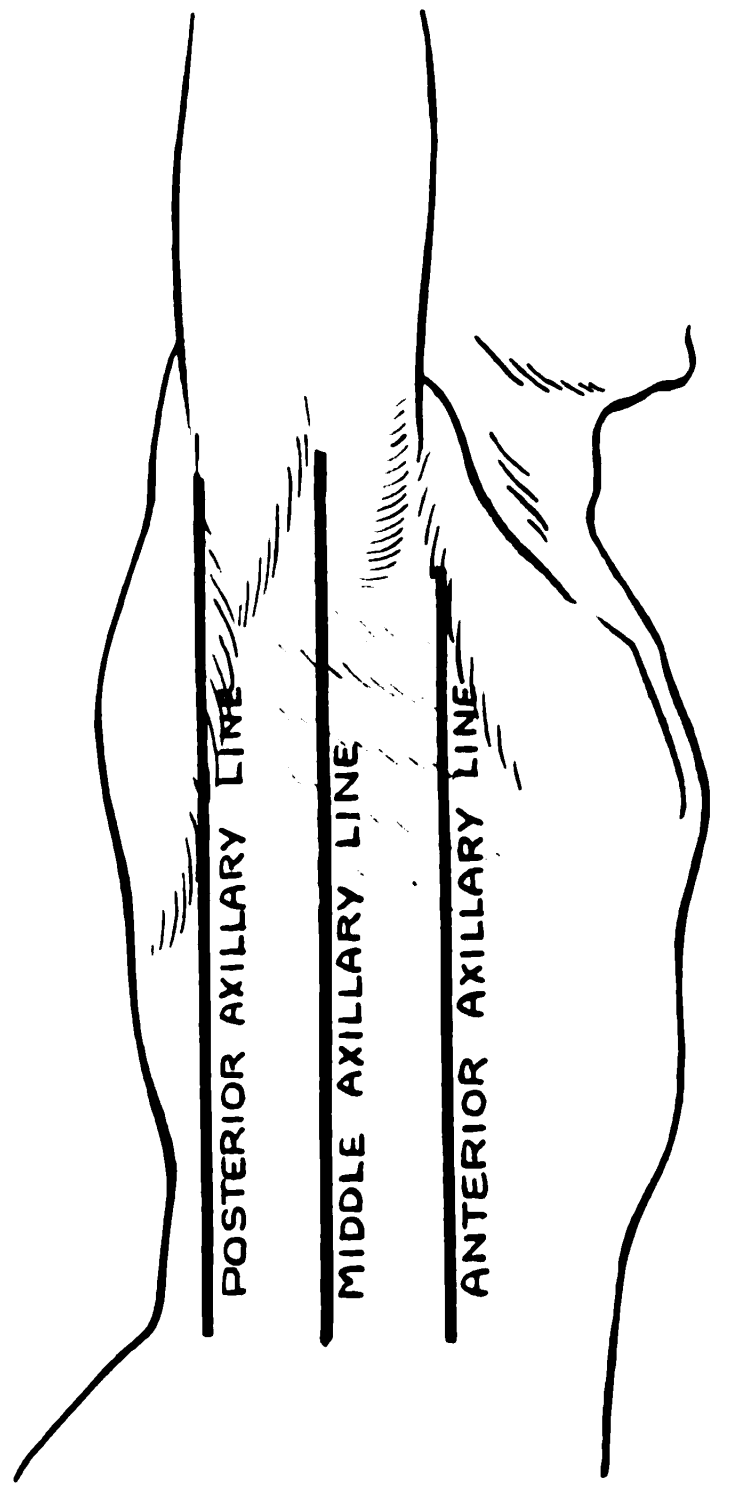
\includegraphics[width=\textwidth,height=6cm,keepaspectratio=true]{images/Brantigan_1963_1-53.png}
	\caption{
		The axillary lines on the right side of chest, taken from \cite{wiki:aux_lines}.
	}
	\label{fig:axillary_lines}
\end{figure}



\subsubsection{Limb Electrodes}
The 4 limb electrodes are denoted as RA, LA, LL, RL and there respective positions are:

\begin{itemize}
	\item RA - Anywhere on right arm between shoulder and elbow, but avoiding thick muscles.
	\item LA - Symmetric to the RA position, but on left arm
	\item RL - Anywhere on right leg between the torso and the ankle
	\item LL - Symmetric to the RL position, but on left leg
\end{itemize} 

The limb electrodes are shown in Figure ~\ref{fig:limb_leads}

\begin{figure}[htpb]
	\centering
	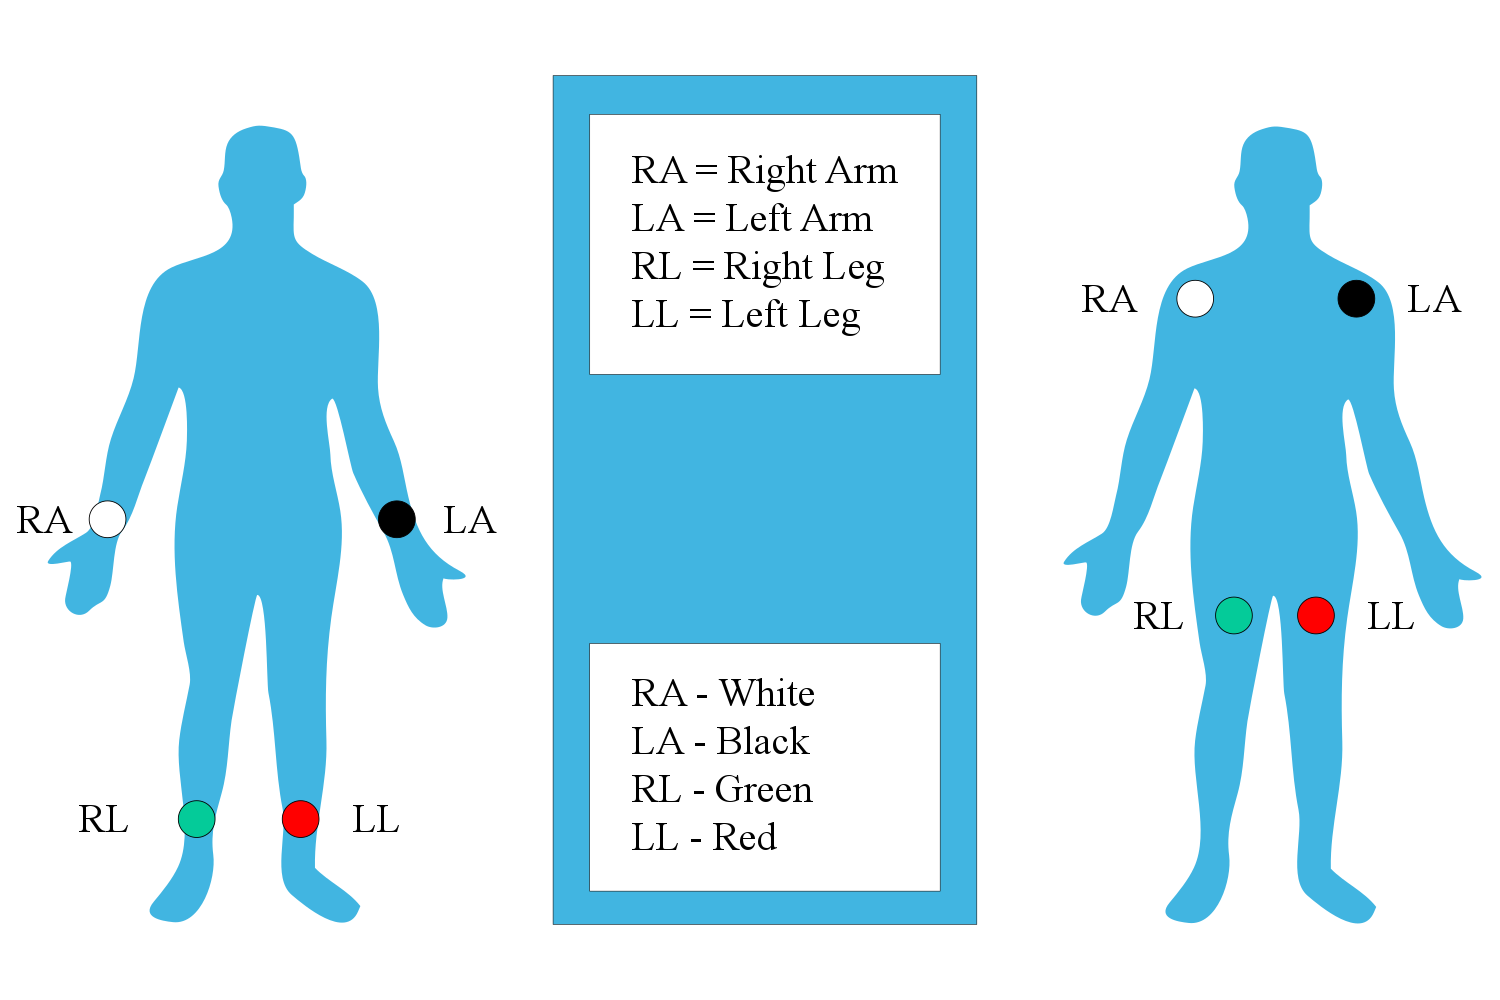
\includegraphics[width=\textwidth,height=6cm,keepaspectratio=true]{images/Limb_leads}
	\caption{
		The possible position of limb leads, taken from \cite{wiki:limb_leads}.
	}
	\label{fig:limb_leads}
\end{figure}


\section{ECG Complex}


ECG complex represents the electrical activity of heart during one cardiac cycle. A normal cardiac cycle consists of five waveforms labeled with P, Q, R, S and T as can be seen in Figure ~\ref{fig:SinusRhythmLabels}. The Q, R and S waves are referred to as one unit, the QRS complex. The ECG signal represents the conduction of electrical impulses from the atria to the ventricles. The important parameters in the ECG signal are:

\subsection{P Wave}

The P wave is the first component of the ECG signal. It occurs due to contraction of the both left and right atrium. This process also known as atrial depolarization. A normal P wave has following characteristics (in lead II):

\begin{itemize}
	\item duration: 0.06 to 0.12 seconds
	\item amplitude: 2 to 3 mm high
	\item location: before the QRS complex
\end{itemize}

\begin{figure}[htpb]
	\centering
	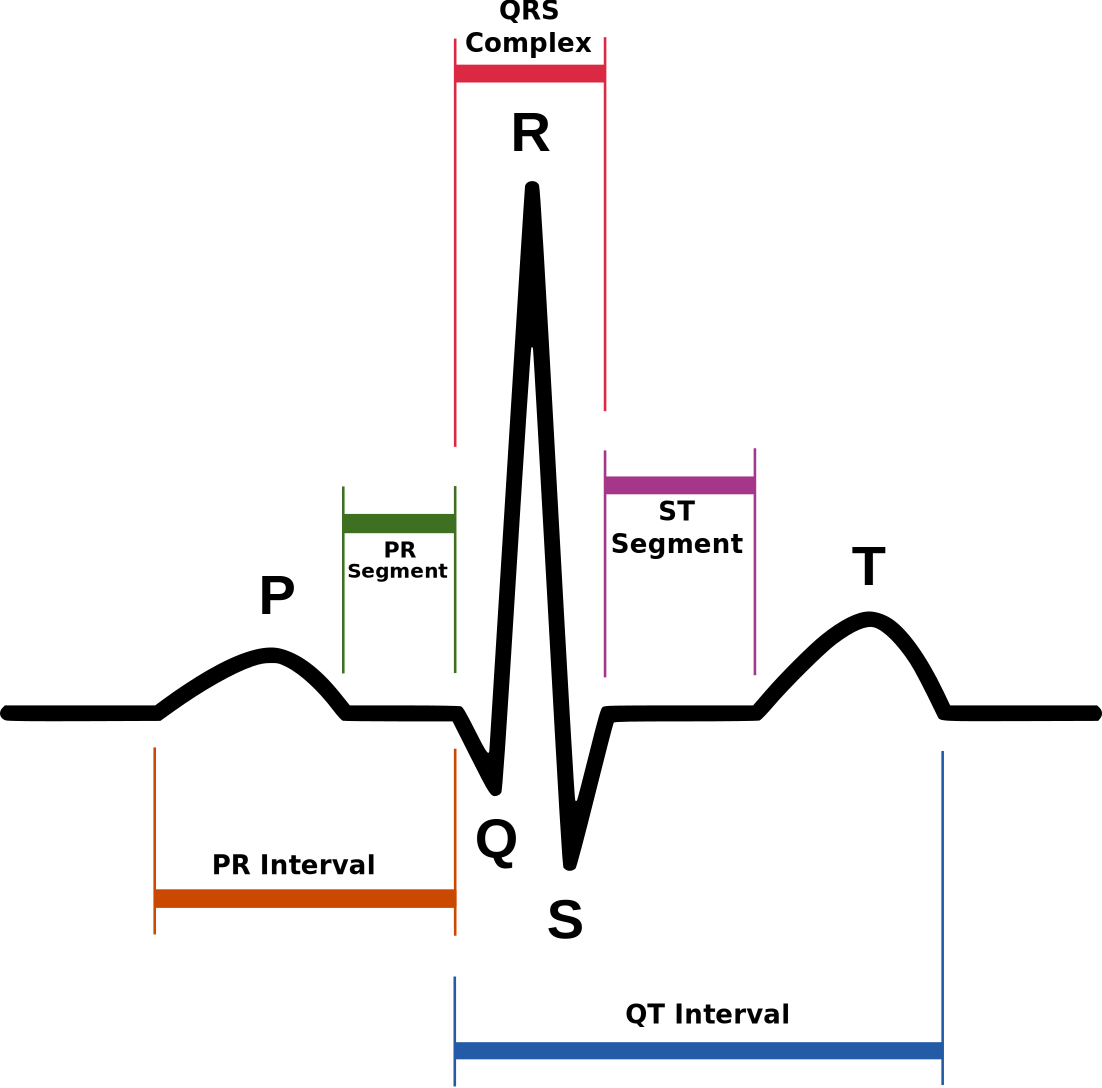
\includegraphics[width=\textwidth,height=6cm,keepaspectratio=true]{images/SinusRhythmLabels}
	\caption{
		The ECG signal, taken from \cite{wiki:SinusRhythmLabels}.
	}
	\label{fig:SinusRhythmLabels}
\end{figure}

\subsection{QRS Complex}
The QRS complex follows the P wave and represents contraction of the both right and left ventricles. This contraction results in the blood ejection from the heart which eventually pumps into the arteries, creating a pulse. The Q and S waves are relatively very small whereas, R wave is comparatively very big. A normal QRS complex has following characteristics (in lead II):

\begin{itemize}
	\item duration: 0.06 to 0.10 seconds
	\item amplitude: 5 to 30 mm high
	\item location: follows the P wave
\end{itemize}

\subsection{T Wave}
The T wave represents the ventricle re-polarization. It occurs during the last part of ventricle systole. The T wave has following characteristics (in lead II):

\begin{itemize}
	\item duration: 0.10 to 0.25 seconds or greater
	\item amplitude: <5 mm high
	\item location: follows the QRS complex
\end{itemize}

\subsection{PR Interval}
The PR interval is the time interval between the end of contraction of the atrium and beginning the contraction of the ventricles. A normal PR interval has following characteristics:

\begin{itemize}
	\item duration: 0.12 to 0.20 seconds
	\item location: From the beginning of P wave to the beginning of the QRS complex
\end{itemize}

\subsection{ST Segment}
The ST segment represents the end of ventricular depolarization and the beginning of the ventricles relaxation. The Point between the end of QRS complex and the beginning of ST segment is called as the J point. A normal ST segment has following characteristics:

\begin{itemize}
	\item duration: 0.08 to 0.12 seconds
	\item location: From the end of QRS complex to the beginning of T wave
\end{itemize}

\subsection{QT Interval}
The QT interval is the time interval between the ventricular depolarization and re-polarization. The QT duration varies according to the heart rate. Faster heart rate results in smaller QT interval whereas, slower heart rate may results in bigger QT interval. The bigger QT interval may results in irregular heart beat. A normal QT interval has following characteristics:

\begin{itemize}
	\item duration: 0.36 to 0.44 seconds
	\item location: From the beginning of QRS complex to the end of T wave
\end{itemize}

\section{Disadvantages of Attached Electrodes} \label{electrodes_disadv}

While it is easy to monitor the electrical heart activity by placing the electrodes directly on the body but it has several disadvantages as well.

\begin{itemize}
	\item It limits the patient's mobility.
	\item Discomfort for the patient as electrodes are directly attached to the body.
	\item Loss of cardiac monitoring in case if patient moves.
	\item Long contact of the electrodes may irritate the skin.
\end{itemize}

\section{Non-Contact ECG}
As described in section \ref{the_electrocardiogram}, the ECG is usually collected by placing electrodes directly on the body but it has several disadvantages as well which is described in section \ref{electrodes_disadv}. Therefore, non-contact capacitive electrodes has been introduced to collect the ECG signals of the patient. Unlike traditional electrodes, which rely on galvanic contact, the capacitive electrodes are insulated from skin using dielectric material, such as, air gap, clothes, etc. The ECG signal propagates via skin to the dielectric material and then to the electrodes through a capacitive coupling.

The major drawback of this approach is that it is very sensitive to body motion.

\section{Noise in ECG Signal}
Most of the time, the ECG signal is corrupted by the different types of noises and artifacts which changes the characteristics of the ECG signal \cite{limaye2016ecg}. Hence, it becomes very difficult to extract the useful information from the signal. Following are the major noises which are present in the ECG signal.

\subsection{Power Line Interference}
Power line interference is a 60 Hz noise which is present in ECG signal because of improper grounding of the ECG equipment or interference from the nearby equipment. In order to remove this type of noise, a proper use of filter is required. A 60 Hz notch filter can be used to remove the power line interference. Figure ~\ref{fig:ACInterference} illustrates the 60 Hz power line interference in ECG signal.

\begin{figure}[htpb]
	\centering
	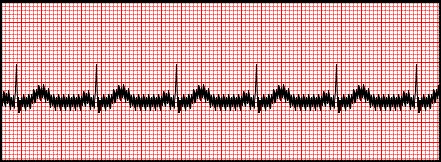
\includegraphics[width=10cm,height=7cm,keepaspectratio=true]{images/ACInterference}
	\caption{
		60 Hz AC Interference, taken from \cite{ecg_artifacts}.
	}
	\label{fig:ACInterference}
\end{figure}

\subsection{Baseline wander}
Baseline wander is a low frequency components which corrupt the ECG signal because of breathing, body movements, dirty or loose electrodes , electrode impedance, etc. Generally they have frequency greater than 1 Hz. A high pass filter can be used to remove the baseline wander. The baseline wandering in ECG signal can be seen in Figure ~\ref{fig:WBaseline}.

\begin{figure}[htpb]
	\centering
	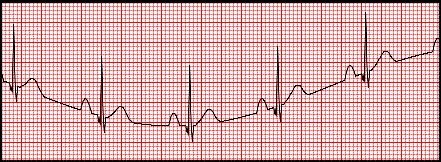
\includegraphics[width=10cm,height=7cm,keepaspectratio=true]{images/WBaseline}
	\caption{
		Baseline wandering in ECG signal, taken from \cite{ecg_artifacts}.
	}
	\label{fig:WBaseline}
\end{figure}

\subsection{Muscle Noise}
This type of noise is caused by muscle contractions besides heart which results in the change of heart electric potential \cite{markovski2013ict}. When the other muscles near the electrodes depolarized and re-polarized, they also generate waves which is then picked up by the ECG. They generally occur in short time burst and have higher amplitude values than the ECG signal. It can be removed using wavelet transform \cite{6091791}. An example of ECG signal effected by muscle contractions can be seen in figure ~\ref{fig:Tremor}.

\begin{figure}[htpb]
	\centering
	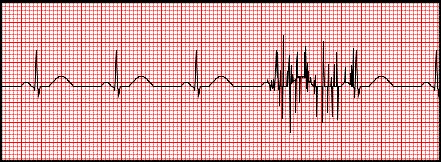
\includegraphics[width=10cm,height=7cm,keepaspectratio=true]{images/Tremor}
	\caption{
		ECG signal combined with muscle noise , taken from \cite{ecg_artifacts}.
	}
	\label{fig:Tremor}
\end{figure}

\section{Arrhythmias}
Irregularity in the heartbeat is known as arrhythmia (also called dysrhythmia) ~\cite{medicinenet}. During arrhythmia, a heart is out of normal rhythm and may feel like the heart is skipped a beat or beat with an irregular pattern. A normal heart rate lies between 60 to 100 beats per miutes and arrhythmia can occur with normal heart rate,  slow heart rate (called bradycardia) in which heart rate 
is less than 60 beats per minute or with rapid heart rate (called tachycardia) in which heart beats faster than 100 beats
per minute.



\subsection{Causes of an Arrhythmia}
Arrhytmia can be caused by one of the following reasons:

\begin{itemize}
	\item Heart disease
	\item Electrolyte imbalance
	\item Changes in heart muscle
	\item After surgery effects
\end{itemize}

\subsection{Types of Arrhythmias}

The most common types of arrhythmias are:

\subsubsection{Premature Ventricular Contraction}
It is a type of arrhythmia in which the heart beat is initiated by the ventricles rather than the SA node. It is is generally refers as "skipped beats". This is the most common type of arrhythmia which occurs with or without any heart disease. It could be the result of too much stress, usage of too much cocaine or restless. But sometimes it can also be caused by heart disease. Most of the time PVC are considered as harmless and rarely need a treatment.

\begin{figure}[htpb]
	\centering
	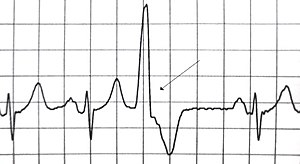
\includegraphics[width=10cm,height=7cm,keepaspectratio=true]{images/pvc}
	\caption{
		Premature Ventricular Contraction, taken from \cite{wiki:pvc}.
	}
	\label{fig:pvc}
\end{figure}

\subsubsection{Atrial Fibrillation}
This type of arrhythmia caused by the abnormal contraction of the upper chamber of heart. During atrial fibrillation, the atria beats irregularly without any coordination with the ventricles. This could results in heart palpation, shortness of breath and weakness.


\subsubsection{Atrial Flutter}
This type of arrhythmia caused by problems in the heart's electrical system. It is similar to atrial fibrillation but rhythm in atria is more organized than the atrial fibrillation. The risk factors and causes of atrial flutter are similar to those of atrial fibrillation.

\begin{figure}[htpb]
	\centering
	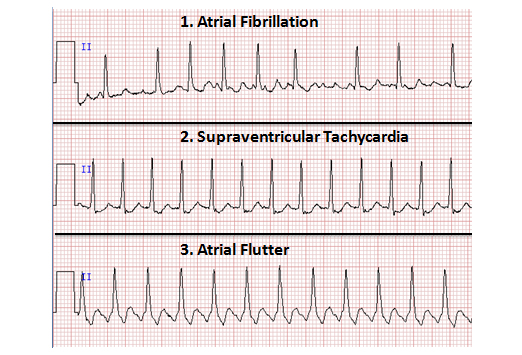
\includegraphics[width=15cm,height=12cm,keepaspectratio=true]{images/af}
	\caption{
		Atrial Fibrillation vs Atrial Flutter vs Tachycardia , taken from \cite{sumdu}.
	}
	\label{fig:af}
\end{figure}


\subsubsection{Bradycardia}
In this type of arrhythmia, the heart beats slower than the normal pace, usually less than 60 beats per minute. This could be because of the disease in electrical heart system.

\subsubsection{Tachycardia}
In this type of arrhythmia, the heart beats faster than the normal pace, usually, more than 100 beats per minute. when the heart beats too fast, it may not pump blood effectively to the body parts, which could result in shortness of breath.

\subsubsection{Heart Block}
In this type of arrhythmia, the heart beats slowly because of the delay or complete block of the electrical signal between the upper chambers and the lower chambers of the heart. It is also called atrial ventricular block (AV block).

\subsubsection{Bundle Branch Block}
Bundle branch block can be of two types, left bundle branch block (LBBB) and right bundle branch block (RBBB). In a normal heart, both bundles depolarized simultaneously and contract at the same time. In this type of arrhythmia, the affected bundle depolarized slowly whereas the un-affected bundle depolarized normally which results in a broader QRS complex, generally longer than 120 milliseconds duration. LBBB and RBBB can be seen in figure ~\ref{fig:LRBBB}.


\begin{figure}[htpb]
	\centering
	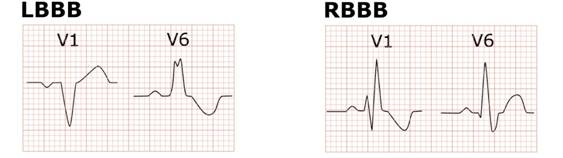
\includegraphics[width=12cm,height=10cm,keepaspectratio=true]{images/LRBBB}
	\caption{
		LBBB vs RBBB , taken from \cite{bilagi}.
	}
	\label{fig:LRBBB}
\end{figure}